% !TEX root = ../zz-lecture.tex


\chapter{动量及其守恒}
动量和能量是高考的重点,也是高中物理课程的重点,同学们平时已经进行了大量的练习。
在本章中,我们对动量的内容进行一些拓展,主要包括二维情况、流体问题及质心系的应用。

\stitle{动量定理}

 在高中课程中我们已经学习过动量定理,并指出动量定理是矢量式,但所研究的问题基本都是一维情况。
 在这个模块中,我们研究一些二维平面问题。
 在应用动量定理时,既可以在某一方向使用,也可以通过正交分解在两个方向上同时使用,即
 \begin{equation}
 	I_i = \Delta p_i,\qquad i=1,2,3
 \end{equation}
 这里的角标$ i $可以理解为矢量在给定直角坐标系中的三个分量值。
 具体方法请大家结合例题学习。
 
 
 \begin{app}{粗糙表面的反弹}{}
 	某小球质量为$ m $,与地面之间的动摩擦系数为$ \mu $,现将小球从高度为$ h $处以初速度$ v_0 $平抛.小球与地面碰撞后,竖直方向的分速度大不变,求小球与地面碰撞后水平方向的分速度大小(假设$ v_0 $很大,小球与地面碰撞后水平方向的分速度不会减为零,且碰撞过程时间极短,重力冲量不计).
 	\tcblower
 	
 	以竖直向上为$ y $轴正方向,初速度$ v_0 $方向为$ x $轴正方向.
 	 	小球落地时竖直方向速度$ v_y = -\sqrt{2gh} $,
 	小球与地面碰撞过程,根据碰撞前后的运动状态变化,对水平、竖直方向分别应用动量定理得:
 	\[
 	I_y=(mv_y)-(-mv_y),\qquad I_x = \mu I_y = mv_x'-mv_0.
 	\]
 	这里已经使用了摩擦力时刻正比于正压力的事实,将以上两式联立不难得到弹起的水平速率
 	\[
 	v_x' = v_0-2\mu\sqrt{2gh}.
 	\]
 
 	
 \end{app}
 
 \begin{example}
 	%%%%题干
 	一袋面粉(可看做质点)沿着与水平面成$ \alpha = \deg{60} $角的光滑斜面,从高$ H $处无初速地滑下,落到水平地板上(不弹起),碰撞过程时间极短,不计重力冲量,袋与地板之间的动摩擦因数$ \mu = 0.7 $,问袋停在何处?
 	%%%%插图
 	%	\begin{problemfig}
 	%		\includegraphics[width=0.6\linewidth]{image/}
 	%	\end{problemfig}
 	
 	\begin{taggedblock}{student}
 		\vspace*{2cm}
 	\end{taggedblock}
 	
 	
 	%%%%答案
 	\begin{taggedblock}{answer}
 		答案:0.5~\si{m}.
 	\end{taggedblock}
 	
 	
 	%%%%解析
 	\begin{taggedblock}{analysis}
 	\begin{center}
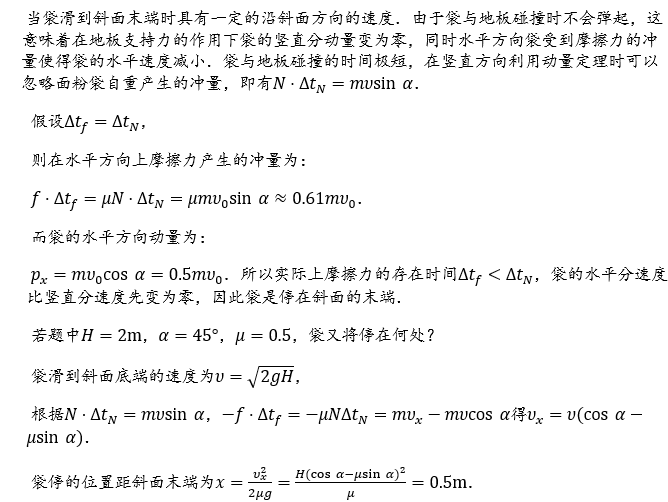
\includegraphics[width=0.8\linewidth]{image/NIR-17}
\end{center}

 	\end{taggedblock}
 \end{example}
 
 \begin{example}
 	%%%%题干
 	 质量足够大的长平板从$ t=0 $时刻开始在水平方向上由静止出发朝右匀加速运动,加速度大小为$ a $.如图所示,在板的上方$ H $高处有一静止的小球,在$ t=0 $时刻自由下落,而后与平板发生碰撞.设小球与平板接触时的滑动摩擦系数$ \mu=0.1 $,小球反弹高度也为$ H $.将小球反弹离开平板时相对地面参考系的速度方向与朝右的水平方向夹角记为$ \beta $,试求$ \tan\beta $与$ a $的关系.(碰撞过程时间极短,重力冲量不计)
 	 
 	 \marginpar{\centering 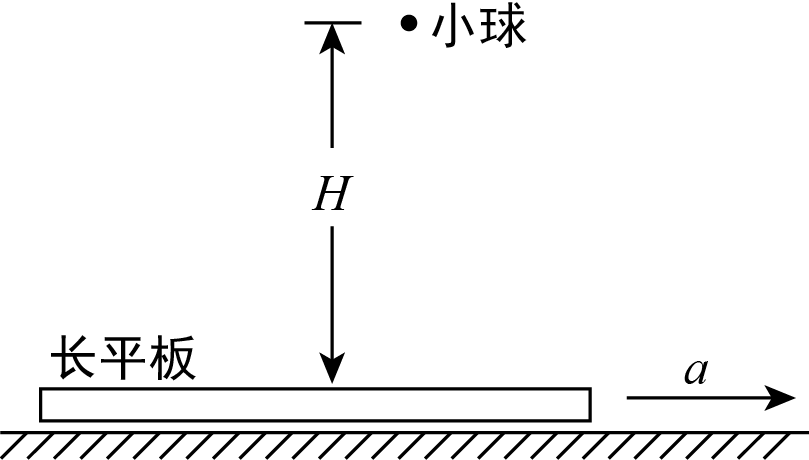
\includegraphics[width=\marginparwidth]{image/momentum-1.png}\figcaption{第\theexample 题 } \label{fig:}}
 	%%%%插图
 	%	\begin{problemfig}
 	%		\includegraphics[width=0.6\linewidth]{image/}
 	%	\end{problemfig}
 	
 	\begin{taggedblock}{student}
 		\vspace*{2cm}
 	\end{taggedblock}
 	
 	
 	%%%%答案
 	\begin{taggedblock}{answer}
 		答案:
 	\end{taggedblock}
 	
 	
 	%%%%解析
 	\begin{taggedblock}{analysis}
 		\begin{center}
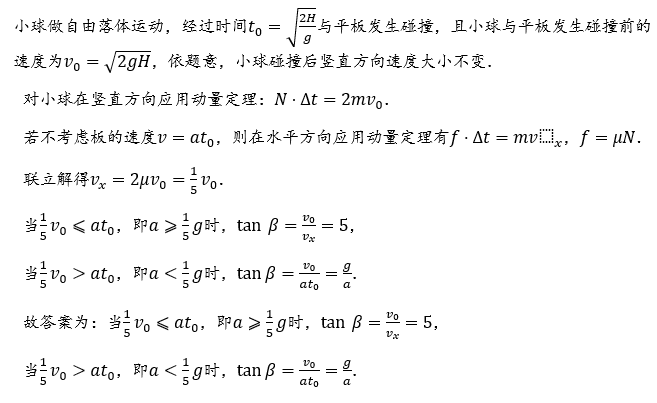
\includegraphics[width=0.8\linewidth]{image/momentum-2}
\end{center}

 	\end{taggedblock}
 \end{example}
 
 
 \begin{example}
 	%%%%题干
 	有一质量及线度足够大的水平板,绕竖直轴以角速度$ \omega $匀速旋转.在板的上方$ h $处有一群相同的小球(可视为质点),它们以板的转轴为中心、$ R $为半径均匀地在水平面内排成一个圆周(以单位长度内小球的个数表示其数线密度).现让这些小球同时从静止状态开始自由落下,设每个球与平板发生碰撞的时间非常;而且碰撞前后小球在竖直方向上速度的大小不变,仅是方向反向;而在水平方向上则会发滑动摩擦,动摩擦因数为$ \mu $.试求这群小球第二次和第一次与平板碰撞时小球数线密度之比值$ \eta $。
 	%%%%插图
 	%	\begin{problemfig}
 	%		\includegraphics[width=0.6\linewidth]{image/}
 	%	\end{problemfig}
 	
 	\begin{taggedblock}{student}
 		\vspace*{2cm}
 	\end{taggedblock}
 	
 	
 	%%%%答案
 	\begin{taggedblock}{answer}
 		答案:
 	\end{taggedblock}
 	
 	
 	%%%%解析
 	\begin{taggedblock}{analysis}
 		 		\begin{center}
 		 			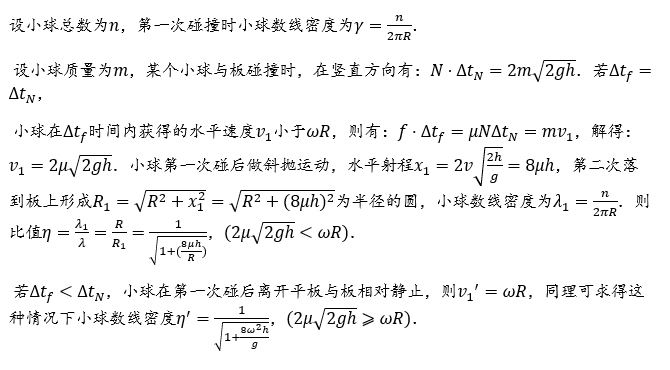
\includegraphics[width=0.8\linewidth]{image/momentum-3}
 		 		\end{center}
 	\end{taggedblock}
 \end{example}
 
 \begin{example}
 	%%%%题干
 	如图所示,完全相同的A、B两个小球质量都为$ m $,放于光滑水平桌面上,两球用质量不计的轻绳连接,绳刚好伸直,现给A球一个与AB连接方向成$ \deg{60} $的瞬时冲量$ I $,求此时B球获得的速度.
 	
 	 	 \marginpar{\centering 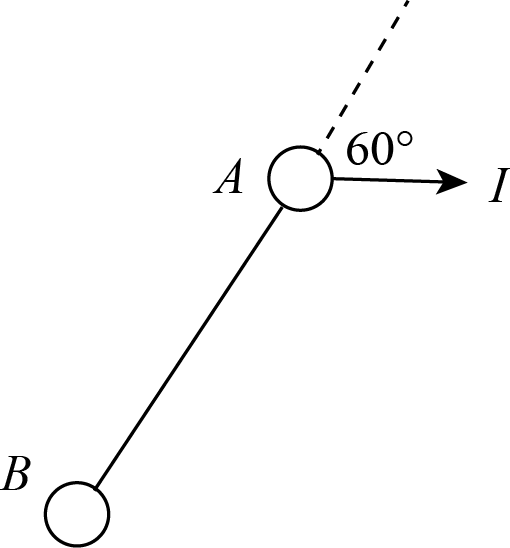
\includegraphics[width=\marginparwidth]{image/momentum-4.png}\figcaption{第\theexample 题 } \label{fig:}}
 	%%%%插图
 	%	\begin{problemfig}
 	%		\includegraphics[width=0.6\linewidth]{image/}
 	%	\end{problemfig}
 	
 	\begin{taggedblock}{student}
 		\vspace*{2cm}
 	\end{taggedblock}
 	
 	
 	%%%%答案
 	\begin{taggedblock}{answer}
 		答案:$ I/4m $
 	\end{taggedblock}
 	
 	
 	%%%%解析
 	\begin{taggedblock}{analysis}
 		解析:	如图所示,	设AB绳子上冲量大小为$ I_1 $,对A、B小球分别沿绳方向应用动量定量,并结合绳两端沿绳方向速度相等可得:
 		\[
 		\frac{I\cos\deg{60}-I_1}{m} = \frac{I_1}{m},
 		\]
 		解得$I_1=1/4 I$,	因为B球速度$ v_B=I_1/m=I/4m $.
 		
 		
 		 \marginpar{\centering 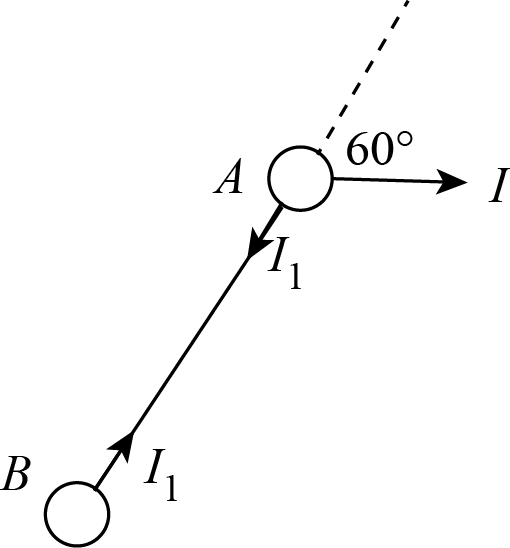
\includegraphics[width=\marginparwidth]{image/momentum-5.png}\figcaption{第\theexample 题 } \label{fig:}}
 	\end{taggedblock}
 \end{example}
 
 \begin{example}
 	%%%%题干
 	 如图所示,质量为$ m $的小球B放在光滑的水平槽内,现有一长为$ l $的细绳连接另一质量为$ m $的小球A,开始细绳处于松弛状态,A与B相距为$ l/2 $,绳子不可伸长,小球A以初速度$ v_0 $向右运动,试求细绳被拉紧时B球的速度$ v_B $.
 	 	 \marginpar{\centering 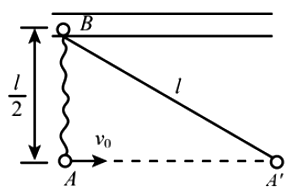
\includegraphics[width=\marginparwidth]{image/momentum-6.png}\figcaption{第\theexample 题 } \label{fig:}}
 	%%%%插图
 	%	\begin{problemfig}
 	%		\includegraphics[width=0.6\linewidth]{image/}
 	%	\end{problemfig}
 	
 	\begin{taggedblock}{student}
 		\vspace*{2cm}
 	\end{taggedblock}
 	
 	
 	%%%%答案
 	\begin{taggedblock}{answer}
 		答案:$ \frac{3}{7}v_0 $
 	\end{taggedblock}
 	
 	
 	%%%%解析
 	\begin{taggedblock}{analysis}
 		解析:设细绳拉紧时绳上冲量为$ I $,则对B球沿水平方向由动量定理
 		\[
 		I\cos\deg{30} = mv_B,
 		\]
 		B球沿绳子速度分量为$v_B\cos\deg{30}$,对A球沿绳方向应用动量定理,并结合绳子两端沿绳方向速度相等,可得$mv_B\cos\deg{30} = mv_0\cos\deg{30}-I$.
 		联立解得  $ I = \frac{2\sqrt{3}mv_0}{7} ,v_B = \frac{3}{7}v_0$.
 	\end{taggedblock}
 \end{example}
 
 \begin{example}
 	%%%%题干
 	如图所示,完全相同的A、B两个小环质量都为$ m $,套在光滑的互相垂直的杆上.整个装置放在光滑水平桌面上,杆固定不动,小环可沿杆无摩擦滑动.两环用质量不计的轻绳连接,开始时绳松弛,给B环沿杆的初速度$ v $,某时刻轻绳张紧,此时绳与B环所在杆成$ \theta $角,求轻绳张紧后瞬间,A球速度.
 	
 		 	 \marginpar{\centering 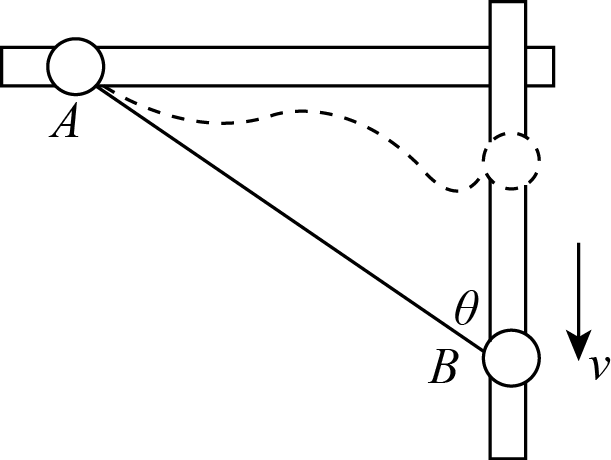
\includegraphics[width=\marginparwidth]{image/momentum-7.png}\figcaption{第\theexample 题 } \label{fig:}}
 	%%%%插图
 	%	\begin{problemfig}
 	%		\includegraphics[width=0.6\linewidth]{image/}
 	%	\end{problemfig}
 	
 	\begin{taggedblock}{student}
 		\vspace*{2cm}
 	\end{taggedblock}
 	
 	
 	%%%%答案
 	\begin{taggedblock}{answer}
 		答案:$ v\cos\theta\sin\theta $
 	\end{taggedblock}
 	
 	
 	%%%%解析
 	\begin{taggedblock}{analysis}
 		解析:\marginpar{\centering 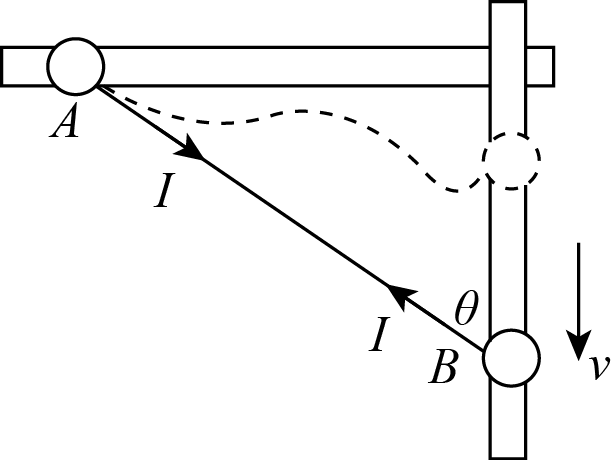
\includegraphics[width=\marginparwidth]{image/momentum-8.png}}
 		\begin{center}
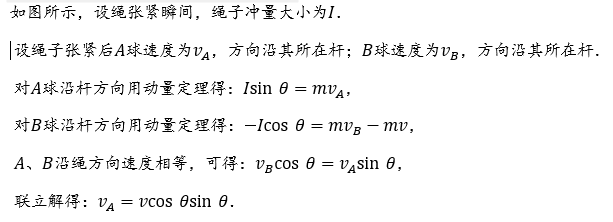
\includegraphics[width=0.8\linewidth]{image/momentum-9}
\end{center}

 	\end{taggedblock}
 \end{example}
 
 
 \begin{example}
 	%%%%题干
 	如图所示,完全相同的A、B两个小球质量都为$ m $,两球用质量不计的轻杆连接,杆与水平方向夹角为$ \deg{53} $,现将两球及轻杆保持图示角度从某高度自由释放,B球与地面接触瞬间,两球速度大小均为$ v $,此后B球与地面发生非弹性碰撞,不从地面弹起,求碰撞后瞬时B球速度.(地面光滑,且碰撞时间极短,忽略重力冲量)
 	 		 	 \marginpar{\centering 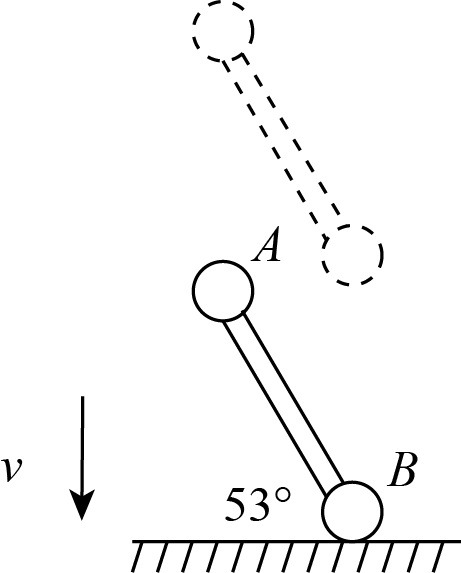
\includegraphics[width=0.8\marginparwidth]{image/momentum-10.png}\figcaption{第\theexample 题 } \label{fig:}}
 	%%%%插图
 	%	\begin{problemfig}
 	%		\includegraphics[width=0.6\linewidth]{image/}
 	%	\end{problemfig}
 	
 	\begin{taggedblock}{student}
 		\vspace*{2cm}
 	\end{taggedblock}
 	
 	
 	%%%%答案
 	\begin{taggedblock}{answer}
 		答案:$\frac{6}{17}v$
 	\end{taggedblock}
 	
 	
 	%%%%解析
 	\begin{taggedblock}{analysis}
 	\begin{center}
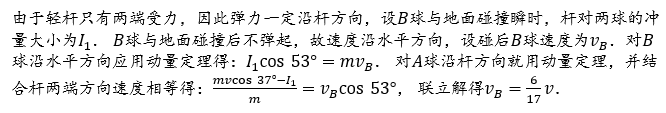
\includegraphics[width=0.9\linewidth]{image/momentum-11}
\end{center}

 	\end{taggedblock}
 \end{example}
 
 
 \begin{example}
 	%%%%题干
 	如图所示,四个质量相等的质点三根不可伸长的绳子依次连接,置于光滑水平面上,三根绳子形成半个正六边形.现有一冲量作用于端点A并使这个质点速度为$ v $,方向沿绳向外,求瞬时D的质点的速度.
 	\marginpar{\centering 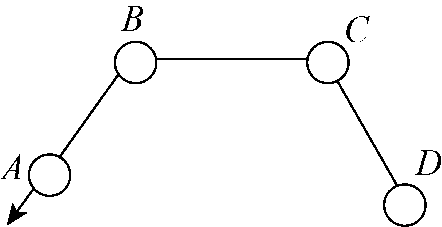
\includegraphics[width=0.8\marginparwidth]{image/momentum-12}\figcaption{第\theexample 题 } }
 	%%%%插图
 	%	\begin{problemfig}
 	%		\includegraphics[width=0.6\linewidth]{image/}
 	%	\end{problemfig}
 	
 	\begin{taggedblock}{student}
 		\vspace*{2cm}
 	\end{taggedblock}
 	
 	
 	%%%%答案
 	\begin{taggedblock}{answer}
 		答案:$ v/13 $
 	\end{taggedblock}
 	
 	
 	%%%%解析
 	\begin{taggedblock}{analysis}
 		解析:
 	\end{taggedblock}
 \end{example}
 
 
 
\stitle{流体的动量}
通常气体流、液体流、不能看成质点的绳子等连续体都可以广义的视为“流体”,在解决与流体有关的问题时,难点和关键点在于如何正确的选取研究对象,这里需要用到微元的思想方法。
通常情况下,我们选择$ \Delta t $时间内流过某一截面的一段流体为研究对象。
然后可以结合动量和能量知识求解,这个模块中我们主要利用动量定理求解。一般思路是:
结合已知条件表示出对应的质量$ \Delta m $(对于光子等问题,可以直接表示出动量);
对该研究对象在$ \Delta t $时间内应用动量定理求解即可(方程中等号两边含有的$ \Delta t $可以最终消掉)。
具体的求解方法请大家结合例题进行学习。


\begin{example}
	%%%%题干
	水力采煤就是利用从高压水枪中喷出来的强力水柱冲击煤层而使煤层碎裂,设所用水枪出水口的横截面积为$ S $,水速为$ v_0 $,水平射到煤层上后水的速度变为0,水的密度为$ \rho $,水柱垂直地冲击到竖直煤壁上后沿竖直煤壁流下,求水柱施于煤层上的冲力大小.
	%%%%插图
	%	\marginpar{\centering \includegraphics[width=0.8\marginparwidth]{image/}\figcaption{第\theexample 题 } }
	
	\begin{taggedblock}{student}
		\vspace*{1cm}
	\end{taggedblock}
	
	
	%%%%答案
	\begin{taggedblock}{answer}
		答案:$ \rho S v^2 $
	\end{taggedblock}
	
	
	%%%%解析
	\begin{taggedblock}{analysis}
		解析:取时间$ t $内的水研究对象,以初速度方向为正方向,根据动量定理,有: $-Ft=0-\rho S v t v$,可得最后结果。
		
	\end{taggedblock}
\end{example}


\begin{example}
	%%%%题干
	某种气体分子束由质量为$ m $速度为$ v $的分子组成,各分子都向同一方向运动,垂直地打在某平面上后又以原速率反向弹回,如分子束每立方米的体积内有$ n $个分子,求被分子束撞击的平面所受到的压强.
	%%%%插图
	%	\marginpar{\centering \includegraphics[width=0.8\marginparwidth]{image/}\figcaption{第\theexample 题 } }
	
	\begin{taggedblock}{student}
		\vspace*{2cm}
	\end{taggedblock}
	
	
	%%%%答案
	\begin{taggedblock}{answer}
		答案:$ 2nmv^2 $
	\end{taggedblock}
	
	
	%%%%解析
	\begin{taggedblock}{analysis}
		解析:设在$ \Delta t $时间内射到面积为S的平面上的气体的质量为$ \Delta m $,则$ \Delta m=v\Delta tSnm $.取Δm为研究对象,它受到的合外力等于平面作用到气体上的压力$ F $.
		以$ ν $方向为正方向,由动量定理得:$ -F\Delta t=(-\Delta mv)-(\Delta mv) $,解得$ F=2v^2 nSm $,平面受到的压强$ p $为:$ p=F/S=2v^2 nm $.
	
		
	\end{taggedblock}
\end{example}

\begin{example}
	%%%%题干
	一个沙漏下部开口面积为$ S $,假设单位时间内漏出沙子的质量保持不变,沙子漏出时的初速度忽略不计,沙漏下部开口距地面高度为$ h $,沙子落地时不反弹,对地面的压强为$ p $,若使沙子落地时对面的压强为$ 2p $,则应使沙漏下部开口距地面高度是多少?
	%%%%插图
		\marginpar{\centering 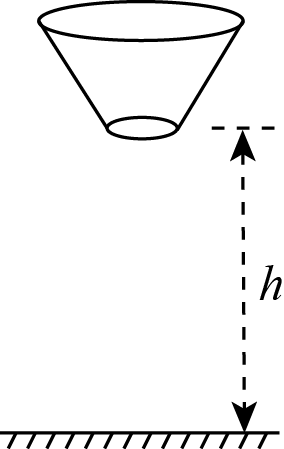
\includegraphics[width=0.6\marginparwidth]{image/momentum-13.png}\figcaption{第\theexample 题 } }
	
	\begin{taggedblock}{student}
		\vspace*{2cm}
	\end{taggedblock}
	
	
	%%%%答案
	\begin{taggedblock}{answer}
		答案:4h
	\end{taggedblock}
	
	
	%%%%解析
	\begin{taggedblock}{analysis}
		解析:由于沙子落地之后不反弹,也就是说,沙子和地面发生的时完全非弹性碰撞,所以不能用能量方程求解,只能列动量冲量方程.
	\end{taggedblock}
\end{example}


\begin{example}
	%%%%题干
	如图所示,电子枪发出的电子初速度忽略不计,电子质量为$ m $,电荷量为$ e $,电子枪与极板间加一加速电压$ U $,电子运动时形成的等效电流为$ I $,电子打到极板上不反弹,求:
	
	1. 电子轰击极板时,对极板的压力.
	2. 若使极板的压力变为2倍,则加速电压应为多少.
	
	%%%%插图
		\marginpar{\centering 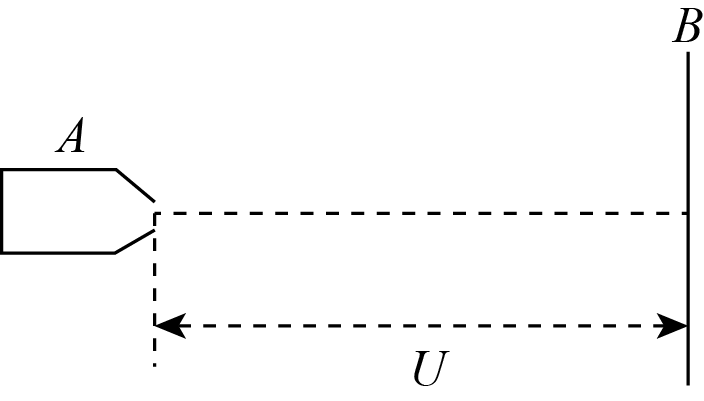
\includegraphics[width=\marginparwidth]{image/momentum-14.png}\figcaption{第\theexample 题 } }
	
	\begin{taggedblock}{student}
		\vspace*{2cm}
	\end{taggedblock}
	
	
	%%%%答案
	\begin{taggedblock}{answer}
		答案:$ 1.I\sqrt{\frac{2mU}{e}} $。 2. $ 4U $
	\end{taggedblock}
	
	
	%%%%解析
	\begin{taggedblock}{analysis}
		解析:
	\end{taggedblock}
\end{example}


\begin{example}
	%%%%题干
	为估算池中睡莲叶面承受水滴撞击产生的平均压强,小明在雨天将一圆柱形水杯置于露台,测得1小时内杯中水上升了\SI{45}{mm}.查询得知,当时雨滴竖直下落速度约为\SI{12}{m/s} .据此估算该压强(设雨滴撞击睡莲后无反弹,不计雨滴重力,雨水的密度为\SI{1e3}{kg/m^3})
	%%%%插图
	%	\marginpar{\centering \includegraphics[width=0.8\marginparwidth]{image/}\figcaption{第\theexample 题 } }
	
	\begin{taggedblock}{student}
		\vspace*{2cm}
	\end{taggedblock}
	
	
	%%%%答案
	\begin{taggedblock}{answer}
		答案:
	\end{taggedblock}
	
	
	%%%%解析
	\begin{taggedblock}{analysis}
		解析:压强$ p = \rho Qv^2 $,其中$ Q $为降雨量。
	\end{taggedblock}
\end{example}

\begin{example}
	%%%%题干
	有一水龙头以每秒\SI{700}{g}水的流量竖直注入盆中,盆放在磅秤上,如图所示,盆中原来无水,盆的质量\SI{500}{g} ,注至10~\si{s}末时,磅秤的读数为\SI{83.3}{N} ,重力加速度为\SI{9.8}{m/s^2},则此时注入盆中的水流的速度是多大?
	%%%%插图
	%	\marginpar{\centering \includegraphics[width=0.8\marginparwidth]{image/}\figcaption{第\theexample 题 } }
	
	\begin{taggedblock}{student}
		\vspace*{2cm}
	\end{taggedblock}
	
	
	%%%%答案
	\begin{taggedblock}{answer}
		答案:\SI{14}{m/s}
	\end{taggedblock}
	
	
	%%%%解析
	\begin{taggedblock}{analysis}
	\begin{center}
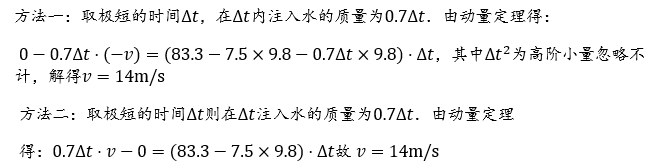
\includegraphics[width=0.8\linewidth]{image/momentum-15}
\end{center}

	\end{taggedblock}
\end{example}


\begin{example}
	%%%%题干
	一质量为$ m $、长为$ l $的均匀柔软绳自由悬垂,下端恰与一台秤秤盘接触.某时刻放开柔软绳上端,求台秤的最大读数.
	%%%%插图
		\marginpar{\centering 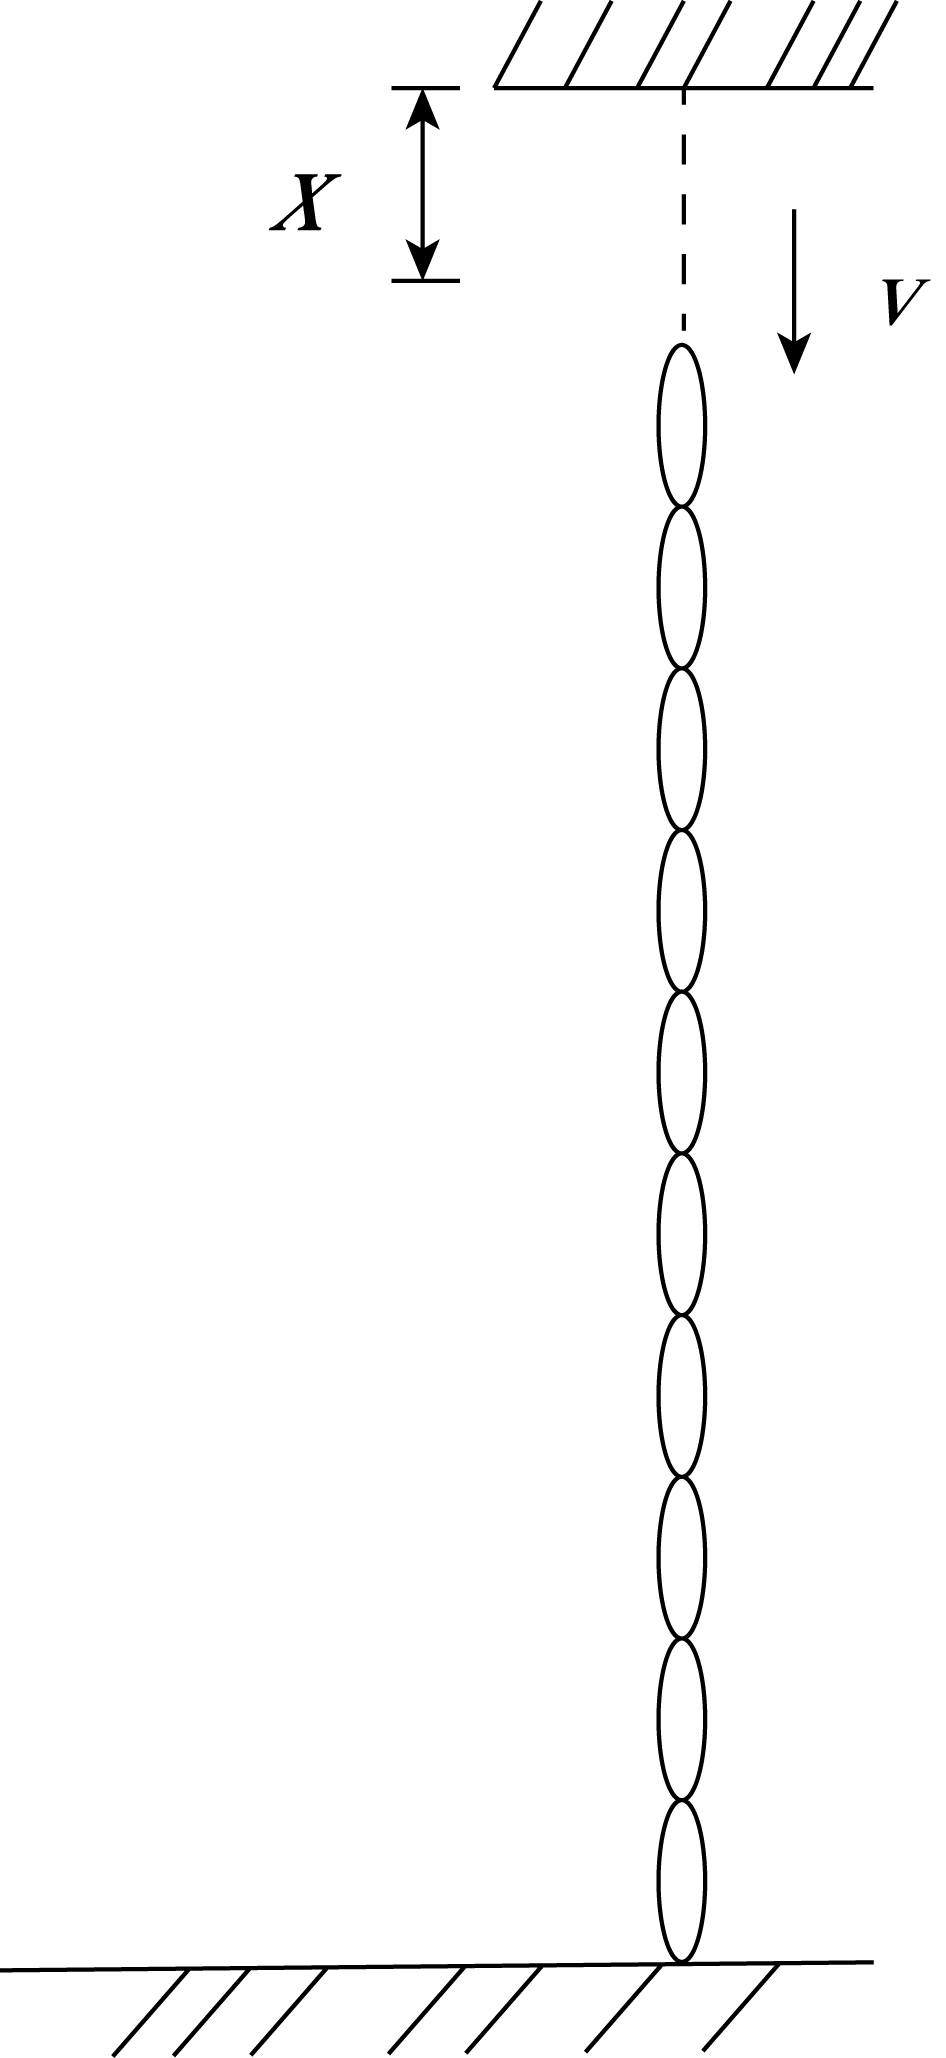
\includegraphics[width=0.4\marginparwidth]{image/momentum-16.png}\figcaption{第\theexample 题 } }
	
	\begin{taggedblock}{student}
		\vspace*{2cm}
	\end{taggedblock}
	
	
	%%%%答案
	\begin{taggedblock}{answer}
		答案:$ 3mg $
	\end{taggedblock}
	
	
	%%%%解析
	\begin{taggedblock}{analysis}
	\begin{center}
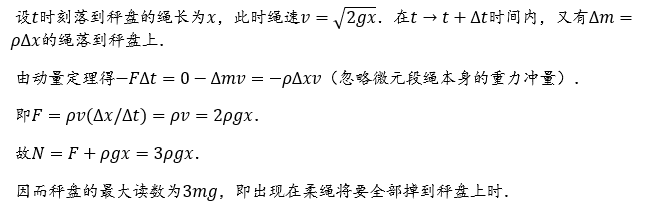
\includegraphics[width=0.8\linewidth]{image/momentum-17}
\end{center}

	\end{taggedblock}
\end{example}


\begin{example}
	%%%%题干
	一帆船在静水中顺风飘行,风速为$ v_0 $,求船速多大时,风供给船的功率最大?(设帆面是完全弹性面,且与风向垂直)
	%%%%插图
	%	\marginpar{\centering \includegraphics[width=0.8\marginparwidth]{image/}\figcaption{第\theexample 题 } }
	
	\begin{taggedblock}{student}
		\vspace*{2cm}
	\end{taggedblock}
	
	
	%%%%答案
	\begin{taggedblock}{answer}
		答案:$ v_0/3 $
	\end{taggedblock}
	
	
	%%%%解析
	\begin{taggedblock}{analysis}
		解析:作用力$ F = 2nmS(v_0-v)^2 $,这样功率
		\[
		P = Fv = 2nmS(v_0-v)^2v,		\]
		上式将在$ v = v_0/3 $处取到极值。
	\end{taggedblock}
	
\end{example}


\begin{example}
	%%%%题干
	由喷泉中喷出的竖直水柱,把一个质量为$ M $的垃圾筒倒顶在空中.若水以恒定的速率$ v_0 $从面积为$ S $的小孔中喷出射向空中,在冲击垃圾筒底后以原速竖直溅下,如图所示,求垃圾筒停留的高度$ h $.
	%%%%插图
		\marginpar{\centering 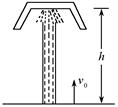
\includegraphics[width=0.7\marginparwidth]{image/momentum-18.png}\figcaption{第\theexample 题 } }
	
	\begin{taggedblock}{student}
		\vspace*{2cm}
	\end{taggedblock}
	
	
	%%%%答案
	\begin{taggedblock}{answer}
		答案:$ h = \frac{1}{2g}\left[ v_0^2-\left( \frac{Mg}{2\rho S v_0} \right)^2  \right]  $
	\end{taggedblock}
	
	
	%%%%解析
	\begin{taggedblock}{analysis}
	\begin{center}
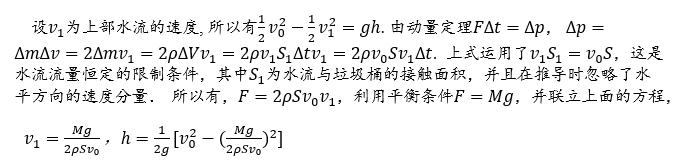
\includegraphics[width=0.9\linewidth]{image/momentum-19}
\end{center}

	\end{taggedblock}
\end{example}

\begin{example}
	%%%%题干
	光子具有能量,也具有动量.光照射到物体表面时,会对物体产生压强,这就是“光压”.光压的产生机理如同气体压强:大量气体分子与器壁的频繁碰撞产生了持续均匀的压力,器壁在单位面积上受到的压力就是气体的压强.设太阳光每个光子的平均能量为$ E $,太阳光垂直照射地球表面时,在单位面积上的辐射功率为$ P_0 $.已知光速为$ c $,则光子的动量为$ E/c $.求:
	
	1. 若太阳光垂直照射在地球表面,则时间t内照射到地球表面上半径为$ r $的圆形区域内太阳光的总能量及光子个数分别是多少?
	
	
	2. 若太阳光垂直照射到地球表面,在半径为r的某圆形区域内被完全反射(即所有光子均被反射,且被反射前后的能量变化可忽略不计),则太阳光在该区域表面产生的光压(用$ p $表示光压)是多少?
	
	
	3. 有科学家建议利用光压对太阳帆的作用作为未来星际旅行的动力来源.一般情况下,太阳光照射到物体表面时,一部分会被反射,还有一部分被吸收.若物体表面的反射系数为$ \rho $,则在物体表面产生的光压是全反射时产生光压的$ (1+\rho)/2 $倍.设太阳帆的反射系数$ \rho=0.8 $,太阳帆为圆盘形,其半径$ r=15~\si{m} $,飞船的总质量$ m=100~\si{kg} $,太阳光垂直照射在太阳帆表面单位面积上的辐射功率$ P_0=1.4~\si{kW} $,已知光速$ c=3\times 10^8~\si{m/s} $ .利用上述数据并结合第2问中的结论,求太阳帆飞船仅在上述光压的作用下,能产生的加速度大小是多少?不考虑光子被反射前后的能量变化.(保留2位有效数字)
	
	
	%%%%插图
	%	\marginpar{\centering \includegraphics[width=0.8\marginparwidth]{image/}\figcaption{第\theexample 题 } }
	
	\begin{taggedblock}{student}
		\vspace*{2cm}
	\end{taggedblock}
	
	
	%%%%答案
	\begin{taggedblock}{answer}
		答案:
	\end{taggedblock}
	
	
	%%%%解析
	\begin{taggedblock}{analysis}
		解析:
	\end{taggedblock}
\end{example}

\stitle{质心运动}

在高中课程中学习动量守恒时,我们碰到过一个常见的模型——人船模型,当时我们是利用动量守恒并结合微元法进行研究的,下面我们利用其他方法再来研究一下这个问题。

在前面的课程中我们学习过质心的概念,质心位置坐标为:
\begin{equation}
x_c = \frac{m_1x_1+m_2x_2+\cdots+m_nx_n}{m_1+m_2+\cdots+m_n},
\end{equation}
若各质点的位移分别为$ \Delta x_1,\Delta x_2,\cdots $,则易知质心位移为:
\begin{equation}
x_c = \frac{m_1\Delta x_1+m_2\Delta x_2+\cdots+m_n\Delta x_n}{m_1+m_2+\cdots+m_n},
\end{equation}
当质点系的动量守恒时,系统所受合外力为零,结合质心运动定律$ \vec{a} = \frac{1}{M}\vec{F^{e}} $,其中$ \vec{F}^{e} $为系统所受的合外力,
可得:$\vec{a}_c=0$,即质心的速度$\vec{v}_c$为常数,质心静止或作匀速直线运动。
因此质心位移$ \Delta x_c=v_c \Delta t $,与上述质心位移公式联立,并结合约束条件即可求得各质点的位移。具体方法请大家结合例题求解。
这种方法的优势在于可以方便地处理初始总动量不为零的问题。

实际上,合外力为零时质心速度不变还可以这样理解:合外力为零时,系统总动量守恒,即$ m_1\vec{v}_1+m_2\vec{v}_2 +\cdots$,又由于$\vec{v}_c  = \frac{1}{M}\sum m_i\vec{v}_i$,因此$ M\vec{v}_c $为常数,它也就是动力学系统的总动量。

\begin{app}{船上的行人}{}
	如图所示,质量为$ M $,长为$ L $的船停在静止的水面上,一质量为$ m $的人(可视为质点)静止站在船头的左端,当人由船头走到船尾,若不计水的阻力,人和船相对于地的位移的大小分别为多少(忽略水对船的阻力,请从质心位移的角度出发求解)?
	\begin{center}

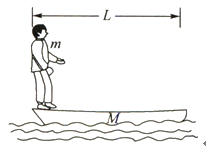
\includegraphics[width=0.4\linewidth]{image/momentum-20}
\end{center}

	\tcblower
	
	“人船模型”是由人和船两个物体构成的系统;该系统在人和船相互作用下各自运动,运动过程中该系统所受到的合外力为零;即人和船组成的系统在运动过程中总动量守恒.
	设人在运动过程中,人和船相对于水面的速度分别为$ v $和$ u $,则由动量守恒定律得$ mv+Mu=0 $
	由于人在走动过程中任意时刻人和船的速度$ v $和$ u $均满足上述关系,所以运动过程中,人和船平均速度大小$ \bar{v} $ 、$\bar{u}$也应满足相似的关系
	\[
	m\bar{v}+M\bar{u}=0.
	\]
	而$ \bar{v} = x/t $,$ \bar{u} = y/t $,其中$ x,y $分别为人和船的位移。
	在此基础上上式可以转化为
	\[
	mx+My = 0.
	\]
	二者相对位移的大小为船的长度$ x+\abs{y} = L $,联立以上几式可得
	\[
	x = \frac{M}{M+m}L,\qquad y = -\frac{m}{M+m}L.
	\]

\end{app}

\begin{example}
	%%%题干
	如图所示,一个质量为$ m $的人(可视为质点)站在长为$ L $、质量为$ M $的船的左端.船在水中以速度$ v $匀速航行(不考虑水的阻力).某时刻人从船的左端向右端走动,经时间$ t $恰好走到船的右端.求此过程中船与人相对地的位移大小分别为多少?
	%%%插图
		\marginpar{\centering 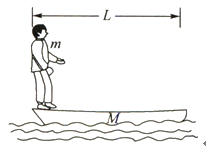
\includegraphics[width=0.8\marginparwidth]{image/momentum-20.png}\figcaption{第\theexample 题 } }
	
	\begin{taggedblock}{student}
		\vspace*{2cm}
	\end{taggedblock}
	
	
	%%%答案
	\begin{taggedblock}{answer}
		答案:人的位移 $ vt+\frac{M}{M+m}L $, 船的位移$ vt-\frac{m}{M+m}L $.
	\end{taggedblock}
	
	
	%%%解析
	\begin{taggedblock}{analysis}
		解析:
	\end{taggedblock}
\end{example}


\begin{example}
	%%%题干
	如图质量分别为$ m_1 $和$ m_2 $的物体A,B静止在光滑水平板上,其间有一被压缩的轻弹簧,长板可以绕O轴转动,另一端用细绳悬于C点.现将弹簧释放,在A、B分别滑向板端的过程中,细绳上的拉力如何变化。
	%%%插图
		\marginpar{\centering 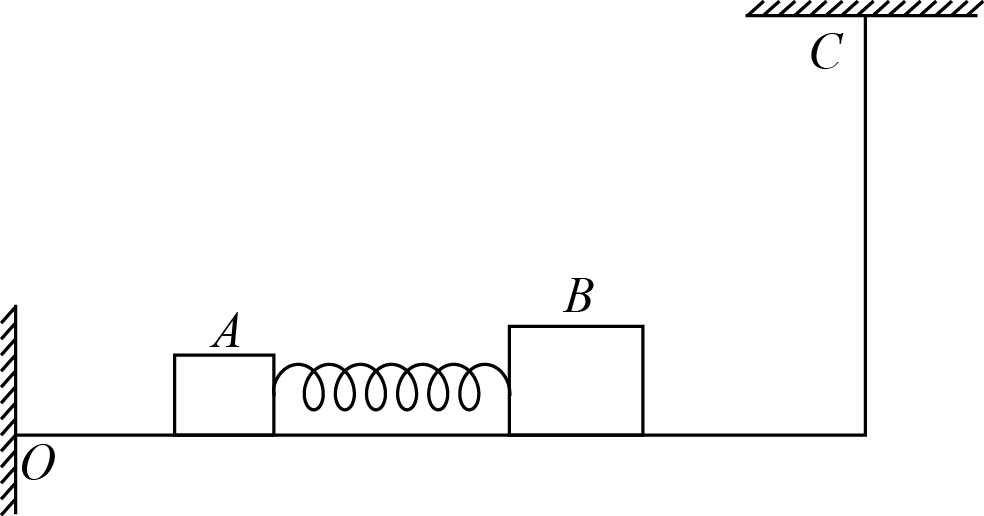
\includegraphics[width=0.8\marginparwidth]{image/momentum-21.png}\figcaption{第\theexample 题 } }
	
	\begin{taggedblock}{student}
		\vspace*{2cm}
	\end{taggedblock}
	
	
	%%%答案
	\begin{taggedblock}{answer}
		答案:不变
	\end{taggedblock}
	
	
	%%%解析
	\begin{taggedblock}{analysis}
		解析:A、B系统水平方向合外力为零,故弹簧伸长的过程中系统质心位置不变,A、B对板的压力相对O点产生的总力矩不变,对板由力矩平衡可知,绳子的拉力大小不变.
	\end{taggedblock}
\end{example}

\begin{example}
	%%%题干
	如图所示,完全相同的物块A、B质量均为$ m $,A、B与劲度系数为$ k $的轻弹簧两端拴接.初始时,弹簧处于压缩状态,压缩量为$ x $,A、B由质量不计的轻绳连接,整个系统以速度$ v $在光滑水平地面上做匀速直线运动.某时刻剪断轻绳,从剪断轻绳到B第一次达到最大速度所用时间为$ t $,求此过程中B对地的位移.
	%%%%插图
		\marginpar{\centering 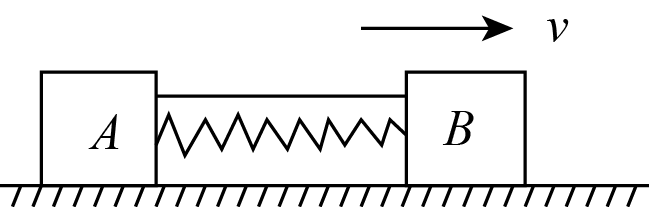
\includegraphics[width=0.8\marginparwidth]{image/momentum-22.png}\figcaption{第\theexample 题 } }
	
	\begin{taggedblock}{student}
		\vspace*{2cm}
	\end{taggedblock}
	
	
	%%%%答案
	\begin{taggedblock}{answer}
		答案:$ vt+\frac{x}{2} $.
	\end{taggedblock}
	
	
	%%%%解析
	\begin{taggedblock}{analysis}
		解析:当B达到最大速度时,从质心系(质心系是惯性系)建立能量守恒方程,得到此时弹簧回到原长.故,B相对质心的位移是$ x/2 $,故此时B对地面的位移为$ vt+x/2 $.
	\end{taggedblock}
\end{example}

\begin{example}
	%%%%题干
	如图所示,质量为$ M $、半径为$ R $的光滑半圆环轨道静止放在光滑水平地面上,质量为$ m $的小球套在圆环轨道上,初始时处于圆环顶端.现在给小球一个微扰(初速度近似为零),小球沿轨道向右滑下.
	
	1. 求小球滑到圆环底端时,水平方向的对地位移; 
	
	2. 如图所示,在初始位置建立相对地面静止的坐标系,求小球下滑过程中的轨迹方程; 
	
	3. 若初始时刻圆环和小球以共同速度v向右做匀速直线运动,小球经时间t滑到圆环底端,求此过程中,小球水平方向的对地位移.
	%%%%插图
		\marginpar{\centering 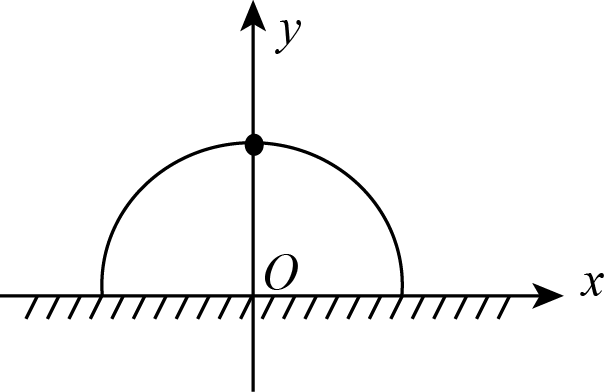
\includegraphics[width=0.8\marginparwidth]{image/momentum-23.png}\figcaption{第\theexample 题 } }
	
	\begin{taggedblock}{student}
		\vspace*{2cm}
	\end{taggedblock}
	
	
	%%%%答案
	\begin{taggedblock}{answer}
		答案:$ 1. \frac{M}{M+m}R;2. (1+\frac{m}{M})^2x^2+y^2 = R^2; 3. vt+\frac{MR}{M+m} $
	\end{taggedblock}
	
	
	%%%%解析
	\begin{taggedblock}{analysis}
		解析:
	\end{taggedblock}
\end{example}

\begin{example}
	%%%%题干
	如图所示,长为\SI{3}{m},质量为\SI{4}{kg}的小车两端的护栏上各装有铁钉,车面光滑且车停在光滑的水平面上.小车内距右端\SI{1}{m} 处放着两个质量分别为$ m_A = \SI{3}{kg},m_B = \SI{2}{kg} $,宽度不计的物块A和B,A、B之间有质量不计、长度不计的压缩弹簧.弹簧释放后B物块获得\SI{4}{m/s}的速度向右运动,两物块碰到钉子后均被钉住,试求小车在整个过程中通过的位移.
	%%%%插图
		\marginpar{\centering 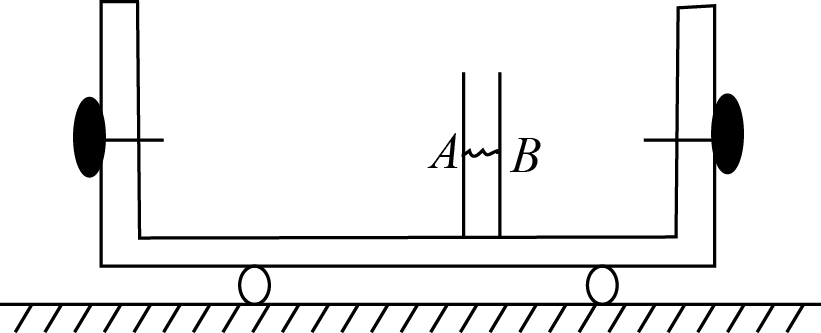
\includegraphics[width=0.8\marginparwidth]{image/momentum-24.png}\figcaption{第\theexample 题 } }
	
	\begin{taggedblock}{student}
		\vspace*{2cm}
	\end{taggedblock}
	
	
	%%%%答案
	\begin{taggedblock}{answer}
		答案:4/9 ~m.
	\end{taggedblock}
	
	
	%%%%解析
	\begin{taggedblock}{analysis}
		解析:
	\end{taggedblock}
\end{example}

\begin{example}
	%%%%题干
	在光滑水平地面上有一凹槽A,中央放一小物块B.物块与左右两边槽壁的距离如图所示,L为\SI{1}{m} .凹槽与物块的质量均为$ m $,两者之间的动摩擦因数$ \mu $为0.05.开始时物块静止,凹槽以$ v_0=\SI{5}{m/s} $初速度向右运动,设物块与凹槽壁碰撞过程中没有能量损失,且碰撞时间不计.g取10\si{m/s^2}.求:
	
	1. 物块与凹槽相对静止时的共同速度.
	
	
	2. 从凹槽开始运动到两者相对静止物块与右侧槽壁碰撞的次数.
	
	3. 从凹槽开始运动到两者相对静止所经历的时间及该时间内凹槽运动的位移大小.
	
	%%%%插图
		\marginpar{\centering 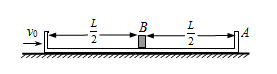
\includegraphics[width=0.8\marginparwidth]{image/momentum-25.png}\figcaption{第\theexample 题 } }
	
	\begin{taggedblock}{student}
		\vspace*{2cm}
	\end{taggedblock}
	
	
	%%%%答案
	\begin{taggedblock}{answer}
		答案:$ 1. v=2.5\si{m/s}; 2. 6; 3. s_2 = 12.75\si{m} $
	\end{taggedblock}
	
	
	%%%%解析
	\begin{taggedblock}{analysis}
		解析:
	\end{taggedblock}
\end{example}